\documentclass[12pt,a4paper,notitlepage]{article}

\usepackage[utf8]{inputenc}

\usepackage[francais]{babel}\usepackage[T1]{fontenc}
\usepackage[cyr]{aeguill}
\usepackage{lmodern}
\usepackage{color}
\usepackage{boites}
\usepackage{caption}
\usepackage{fancybox}
\usepackage{listings}
\usepackage{multicol}

%\lstset{language=bash, basicstyle=\footnotesize, frame=shadowbox, rulesepcolor=\color{gris}, captionpos=b}

  \lstset{
         basicstyle=\footnotesize\ttfamily, % Standardschrift
         %numbers=left,               % Ort der Zeilennummern
         numberstyle=\tiny,          % Stil der Zeilennummern
         %stepnumber=2,               % Abstand zwischen den Zeilennummern
         numbersep=5pt,              % Abstand der Nummern zum Text
         tabsize=2,                  % Groesse von Tabs
         extendedchars=true,         %
         breaklines=true,            % Zeilen werden Umgebrochen
         keywordstyle=\color{red},
                frame=b,         
         keywordstyle=[1]{\itshape}{//},    % Stil der Keywords
         stringstyle=\color{white}\ttfamily, % Farbe der String
         showspaces=false,           % Leerzeichen anzeigen ?
         showtabs=false,             % Tabs anzeigen ?
         xleftmargin=5pt,
         framexleftmargin=1pt,
         framexrightmargin=5pt,
         %numbers=left,
         frame=toplines,
         framextopmargin=3pt,
       %  framexleftmargin=8pt,
         numberblanklines=false,
         %morecomment=[s][marron]{/*}{*/},
         %moredelim=*[s][\color{blue}]{/*}{*/}
         %morecomment=[s][marron]{/*-}{*/}},         
         framexbottommargin=5pt,
         captionpos=b,
         %backgroundcolor=\color{lightgray},
         showstringspaces=false      % Leerzeichen in Strings anzeigen ? 
 }

\DeclareCaptionFont{white}{\color{white}}
\DeclareCaptionFormat{listing}{\colorbox[cmyk]{0.43, 0.35, 0.35,0.01}{\parbox{\textwidth}{\hspace{10pt}#1#2#3}}}
\captionsetup[lstlisting]{format=listing,labelfont=white,textfont=white, singlelinecheck=false, margin=0pt, font={bf,footnotesize}}

\definecolor{gris}{gray}{0.75}
%\definecolor{bleup}{HTML}{258EE9}


%\renewcommand*\familydefault{\ttdefault} %% Only if the base font of the document is to be typewriter style
%\renewcommand{\rmdefault}{ptm}


\usepackage[
   pdfauthor={Ludovic Terrier & Arnaud Goulut},
   pdftitle={RE12 - TP5},
   ]{hyperref}
   
   
\usepackage[pdftex]{graphicx}

%\usepackage{titlesec}
%\titleformat{\section}[frame] {\normalfont} {\filright
%\footnotesize
%\enspace\textbf{\thesection}\enspace} {8pt} {\Large\bfseries\filcenter}

%% Je contrôle la taille de ma zone imprimée...
\usepackage{anysize}
%% ...en définissants les marges {gauche}{droite}{haute}{basse}
\marginsize{25mm}{15mm}{10mm}{15mm}

\begin{document}

\title{Mise en \oe uvre d'une infrastructure de ToIP}
\author{Arnaud Goulut et Ludovic Terrier}
\date{Juin 2010}
\maketitle


%\tableofcontents

\thispagestyle{empty}


 
%%%%%%%%%%%%%%%%%%%%%%%%%%%%%%%%%%% 1ère partie
\section{Etude théorique}
\subsection{SIP}
\subsection{messages}

\section{Architecture utilisée}
\subsection{configuration réseau}
\subsection{configuration téléphone}

\section{Fichiers de configuration SIP}
\subsection{sip.conf}
\subsection{extensions.conf}

\section{IAX} 
\subsection{pourquoi?}
\subsection{fichier IAX.conf}

\section{Fichiers de traces}
\subsection{message INVITE (en détail)}
\subsection{message BYE} 


\noindent \texttt{user@machine  chmod +x LdapAdminTool-4.6.1.x-Linux-x86-Install.bin \\
user@machine  ./LdapAdminTool-4.6.1.x-Linux-x86-Install.bin}
\bigskip

\begin{figure}[!h]
\begin{center}
%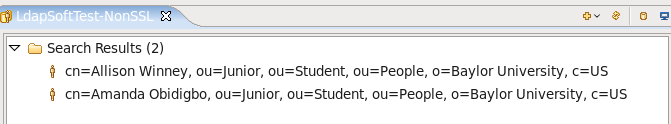
\includegraphics[scale=0.61]{recherche}
\caption{Résultat d'une recherche dans LDAP Admin Tools.}
\label{fig:da}
\end{center}
\end{figure}




\end{document}